\chapter{Aplicaciones continuas}%
\label{cha:aplicaciones_continuas}


\section{Continuidad}%
\label{sec:continuidad}
El famoso $\varepsilon-\delta$ en $\mathbb{R}^n\ \mathcal{T}_u,\ x_0 \in X,\ f : \overbrace{X}^{\subset \mathbb{R}^p} \rightarrow \overbrace{Y}^{\subset \mathbb{R}^q}$: 
\begin{gather*}        
\forall \varepsilon > 0, \exists \delta > 0: 
\begin{cases}
    \lVert x - x_0 \rVert < \delta \Rightarrow \lVert f\left( x \right) - f\left( x_0 \right) \rVert < \varepsilon \Leftrightarrow\\
    x \in B\left( x_0, \delta \right) \Rightarrow f\left( x \right) \in B\left( f\left( x_0 \right), \varepsilon \right) \Leftrightarrow\\
    f\left( B\left( x_0, \delta \right) \right) \subset B\left( f\left( x_0 \right), \varepsilon \right) 
\end{cases} \Rightarrow\\
\boxed{\forall B\left( f\left( x_0 \right), \varepsilon \right),\ \exists B\left( x_0, \delta \right) \subset f^{-1}\left( B\left( f\left( x_0 \right), \varepsilon \right) \right)} 
.\end{gather*}

\begin{defi}
$f: X \rightarrow Y$ será \underline{continua en $x_0$} $\in X$ si: 
\[
\forall V^{f\left( x_0 \right)}: f^{-1}\left( V^{f\left( x_0 \right)} \right) = V^{x_0},
\]
es decir, $f^{-1}\left( V^{f\left( x_0 \right)} \right)$ será entorno de $x_0$.
\end{defi}

\begin{prop}[Composición de continuidades]
La composición de funciones continuas es continua:

\[
X \xrightarrow{f} Y \xrightarrow{g} Z: \begin{rcases}
    f \text{ continua en } x_0\\
    g \text{ continua en } y_0
\end{rcases} \Rightarrow h = g \circ f \text{ continua en }  x_0
\]
\end{prop}
\begin{demo}
Sea $V^{h\left( x_0 \right)} \rightarrow h^{-1} V^{h\left( x_0 \right)} = f^{-1}g^{-1}V^{g\left( y_0 \right)} = f^{-1} V^{y_0} = V^{x_0}$. Por las continuidades de $g$ y $f$.
\end{demo}

\begin{defi}
$f: X \rightarrow Y$ es \underline{continua} si lo es en todos los puntos de su dominio.
\end{defi}

\begin{ej}
\begin{enumerate}
    \item $\forall f: X_{\text{discreta}} \rightarrow Y$ es continua. 
    \begin{demo}
        Todo es abierto, luego todo es entorno en $\mathcal{T}_{\text{disc}}$.
    \end{demo}
    \item $\forall f: X \rightarrow Y_{\text{trivial}}$ continua. 
    \begin{demo} 
        $V^{f\left( x \right)} = Y$ es el único abierto, luego el único entorno, de $f^{-1}V^{f\left( x \right)} = f^{-1}Y = X$ es abierto.
    \end{demo}
    \item $f: X \rightarrow Y_{\text{discreta}}$ es continua $\Rightarrow f$ localmente constante.
    \begin{demo}
        $\{f\left( x_0 \right)\} = V^{f\left( x_0 \right)}$ en $\mathcal{T}_{\text{discr}} \xRightarrow[f\text{ cont.}]{} f^{-1}f\left( x_0 \right) = V^{x_0}\; \land \;f \equiv f\left( x_0 \right),\ \forall x \in V^{x_0}$.
    \end{demo}
    \item $f: X \rightarrow Y$ localmente constante $\Rightarrow$ continua.
    \begin{demo}
        $\forall x_0 \in X,\ \exists U^{x_0} : f \stackrel{U^{x_0}}{\equiv} f\left( x_0 \right) \Rightarrow \forall V^{f\left( x_0 \right)}: f^{-1}V^{f\left( x_0 \right)} \supset U^{x_0} \Rightarrow f^{-1}V^{f\left( x_0 \right)} = V^{x_0}$ es entorno de $x_0$.
    \end{demo}
\end{enumerate}
\end{ej}

\begin{prop}
Son equivalentes:
\begin{enumerate}
    \item $f$ es continua.
    \item $f^{-1}\left( \text{abierto}  \right) = \text{abierto} ,\ \forall \text{abierto} \in Y$.
    \item $f^{-1}\left( \text{cerrado} \right) = \text{cerrado},\ \forall $ cerrado de $Y$.
    \item $f^{-1}\left( \mathring{A} \right) \subset \inter\left( f^{-1}\left( A \right) \right),\ \forall A \subset Y$
    \item $f\left( \overline{A} \right) \subset \overline{f\left( A \right)},\ \forall A \subset X$. 
\end{enumerate}
\end{prop}
\begin{demo}
\begin{enumerate}
    \item $1 \Rightarrow 2)$
    \[
        W \stackrel{\text{ab.}}{\subset}  Y \Rightarrow W \text{ ent. de } f\left( x \right),\ \forall x \in f^{-1}W \xRightarrow{f \text{cont.}} f^{-1} W \text{ ent. } \forall x \in f^{-1}W \Rightarrow f^{-1} W \stackrel{\text{ab.}}{\subset}  X 
    \]
    \item $2 \Rightarrow 3)$
    \[
        C \stackrel{\text{cerr.}}{\subset}  Y \Rightarrow Y \setminus C \stackrel{\text{ab.}}{\subset} Y \Rightarrow^{2)} \underbrace{f^{-1}\left( Y\setminus C \right)}_{= X \setminus f^{-1}C} \stackrel{\text{ab.}}{\subset} X \Rightarrow f^{-1}C \stackrel{\text{cerr}}{\subset} X 
    \]
    \item $3 \Rightarrow 5)$

    \[
        \overline{f\left( A \right)} \stackrel{\text{cerr}}{\subset} Y \Rightarrow^{3)} \underbrace{f^{-1}\overline{f\left( A \right)}}_{\supset f^{-1}f\left( A \right) \supset A} \stackrel{\text{cerr.}}{\subset} X \Rightarrow \overline{A} \subset f^{-1}\overline{f\left( A \right)} \Rightarrow f\left( \overline{A} \right) \subset \overline{f\left( A \right)} 
    \]
    \item $5 \Rightarrow 4)$
    \begin{gather*}
        Y \setminus \mathring{A}\Rightarrow \overline{Y\setminus A} \supset \overline{f\left( X \setminus f^{-1}A \right)} \stackrel{5)}{\supset} f\left( \overline{X \setminus f^{-1}\left( A \right)} \right) = f\left( X \setminus \inter\left( f^{-1}A \right) \right) \Rightarrow\\
        X \setminus \inter\left( f^{-1}A \right) \subset f^{-1}\left( Y\setminus \mathring{A} \right) = X \setminus f^{-1}\left( \mathring{A} \right)\stackrel{c}{\Rightarrow}  f^{-1}\left( \mathring{A} \right) \subset \inter\left( f^{-1}A \right) 
    .\end{gather*}

    \item $4 \Rightarrow 1)$
    \begin{gather*}
        V^{f\left( x \right)} \Rightarrow f\left( x \right) \in \inter\left( V^{f\left( x \right)} \right) \Rightarrow x \in f^{-1}\left( \inter\left( V^{f\left( x \right)} \right) \right) \subset \inter\left( f^{-1}V^{f\left( x \right)} \right) \Rightarrow \\
        f^{-1}V^{f\left( x \right) } \text{ entorno de } x.
    \end{gather*}
\end{enumerate}
\end{demo}

\begin{obs}
\begin{enumerate}
    \item Los cuatros primeros enunciados tratan sobre ``imágenes inversas''. Por ejemplo, la segunda dice que $f^{-1}\mathcal{T}_Y \subset \mathcal{T}_X$.
    \item Pensando que un punto adherente es un ``punto límite'', $5$ nos dice que ``la imagen del límite es el límite de la imagen''.
    \item $id: \left( X, \mathcal{T}_1 \right) \rightarrow \left( X, \mathcal{T}_2 \right)$ es continua $\Rightarrow \mathcal{T}_2 \subset \mathcal{T}_1$. 
    \begin{demo}
        $id^{-1}\mathcal{T}_1 = \mathcal{T}_2$.
    \end{demo}
\end{enumerate}
Y no mencionamos todos los ejemplos conocidos en espacios afines $\mathbb{R}^n$ con $\mathcal{T}_u$.
\end{obs}


\section{Continuidad y subespacios}%
\label{sec:continuidad_y_subespacios}
\begin{prop}
Sea $f: X \rightarrow Y$ continua y $Z \subset X$ un subespacio $\Rightarrow f|_Z : Z \rightarrow Y$ es continua.
\end{prop}
\begin{demo}
Se aplica el criterio ``imagen inversa de abierto es abierto'' y la fórmula:
\[
\left( f|_Z \right)^{-1} \left( A \right) = Z \cap f^{-1}A,\ \forall A \subset Y
\]
que es abierta por definición de abierta en una restricción.
\end{demo}

%TODO: Diagramas composición
\begin{obs}
\begin{enumerate}
    \item $Z \stackrel{j}{\subset} X$ es continua.
    \begin{demo}
        \begin{itemize}
            \item $z \in Z: \forall V^{j\left( z \right)} : \underbrace{j^{-1}\left( V^{j\left( z \right) } \right)}_{= V^{j\left( z \right)} \cap Z}$ entorno de $z$ en $Z$.
            \item $\forall U \stackrel{\text{ab.}}{\subset } X: \underbrace{j^{-1}\left( U \right)}_{U \cap Z} \stackrel{\text{ab.}}{\subset} Z$
        \end{itemize}
    \end{demo}

    \item $Z \stackrel{j}{\subset} X \xrightarrow{f} Y$. Si $f$ es cont. $\Rightarrow f|_Z$ continua. (No a la inversa).
    \begin{demo}
    Como $f|_Z = f \circ j$ y ambas son continuas, por composición, $f|_Z$ es continua.
    \end{demo}

    \item La continuidad es \underline{local}. 

    Si $f|_{E^x}$ continua en $x \Rightarrow f$ continua en $x$.
    \begin{demo}
        $\forall V^{f\left( x \right)} \Rightarrow \left( f|_{E} \right)^{-1}\overbrace{\left( V^{f\left( x \right)} \right)}^{= W^x}$ entorno de $x$ en $E^x$.

        Como $W^x \stackrel{\text{ent.}}{\subset} E^x \stackrel{\text{ent.}}{\subset} X$ (entorno en entorno es entorno). Porque, 
        \[
        \begin{rcases}
            x \in W^x: \exists G \stackrel{\text{ab.}}{\subset} W^x \subset E^x: G = A \cap E^x \subset X\\ 
            x \in E^x: \exists B \stackrel{\text{ab.}}{\subset} E^x \subset X 
        \end{rcases} \Rightarrow x \in \underbrace{A \cap B}_{\stackrel[\text{ab.}]{}{\subset} X} \subset \underbrace{A \cap E^x}_{= G}  \subset W^x
        \]
    \end{demo}

    \item Si $f|_{U \stackrel{\text{ab.}}{\subset} X}$ es continua $\Rightarrow f$ continua $\forall x \in U$.

    \item $x$ es aislado $\Rightarrow f$ continua en $x$. 
    \begin{demo}
        $x$ aislado $\Leftrightarrow V^x = \{x\}$ es abierto de $X$. $f|_{V^x} : \{x\} \rightarrow Y$.
    \end{demo}

    \item $f: X \rightarrow Y \supset Z$ tal que $f\left( X \right) \subset Z \subset Y$ (si no es así puede estar mal definido).

    Entonces, $f$ a $Y$ es continua $\Leftrightarrow f$ a $Z$ es continua.
    \begin{demo}
        \begin{itemize}
            \item $f$ cont. en $Z \xRightarrow{j \circ f} f$ cont. en $Y$.
            \item $f$ cont. en $Y \xRightarrow{?} f$ cont. en $Z$. 

            Sea $U_z$ ab. en $Z$. Este será $U_y \cap Z = U_z$ que cumple, $f_z^{-1}\left( U_y \cap Z \right) \stackrel{f\left( X \right) \subset Z}{=}  f_y^{-1}\left( U_y \right)$ que es abierto en $X$ (por ser $f_y$ continua).
        \end{itemize}
    \end{demo}
\end{enumerate}
\end{obs}

\begin{prop}[Criterios de continuidad por recubrimientos]
Sea $f: X \rightarrow Y$ será continua sii:
   \begin{itemize}
        \item \textbf{Por abiertos:} $\exists X = \bigcup_{i \in  I} U_i^{\text{ab.}}: \forall f|_{U_i} : U_i \rightarrow Y$ es continua. 

        \item \textbf{Por cerrados:} $\exists X = \bigcup_{i = 0}^{n} F_i^{\text{cerr.}}: \forall f|_{F_i} : F_i \rightarrow Y$ es continua. 
   \end{itemize} 
\end{prop}
\begin{demo}
\begin{itemize}
    \item $W \stackrel{\text{ab.}}{\subset} Y \Rightarrow$
    \[
    \begin{cases}
        f^{-1}W = \bigcup_{i \in  I} U_i \cap f^{-1} W = \bigcup_{i \in  I} \left( f|_{U_i} \right)^{-1} W\\
        \left( f|_{U_i} \right)^{-1}W \stackrel[\text{(cont.)}]{\text{ab.}}{\subset} U_i \stackrel{\text{ab.}}{\subset} X \Rightarrow \left( f|_{U_i} \right)^{-1} W \stackrel{\text{ab.}}{\subset} X
    \end{cases}\Rightarrow f^{-1}W \stackrel{\text{ab.}}{\subset} X  
    \]
    Por unión de abiertos.

    \item $C \stackrel{\text{cerr.}}{\subset} Y \Rightarrow$
    \[
    \begin{cases}
        f^{-1}C = \bigcup_{i = 0}^{n}  F_i \cap f^{-1} C = \bigcup_{i = 0}^{n} \left( f|_{F_i} \right)^{-1} C\\
        \left( f|_{F_i} \right)^{-1}C \stackrel[\text{(cont.)}]{\text{cerr.}}{\subset} F_i \stackrel{\text{cerr.}}{\subset} X \Rightarrow \left( f|_{F_i} \right)^{-1} C \stackrel{\text{cerr.}}{\subset} X
    \end{cases}\Rightarrow f^{-1}C \stackrel{\text{cerr.}}{\subset} X  
    \]
    Por unión finita de cerrados.
\end{itemize}
\end{demo}

\begin{defi}[Aplicaciones continuas por recubrimientos]
\begin{itemize}
    \item Por \underline{abiertos}: $\{f_i: U_i \xrightarrow{\text{cont.}} Y\}_{i \in I}$. Donde $X = \bigcup_{i \in I} U_i$. 

    $\exists f: X \rightarrow Y \Leftrightarrow f_i|_{U_i \cap U_j} = f_j|_{U_i \cap U_j}$.

    \item Por \underline{cerrados}: $\{f_i: F_i \xrightarrow{\text{cont.}} Y\}_{i = 1}^n$. Donde $X = \bigcup_{i = 1}^n F_i$. 

    $\exists f: X \rightarrow Y \Leftrightarrow f_i|_{F_i \cap F_j} = f_j|_{F_i \cap F_j}$.
\end{itemize} 
\end{defi}


\section{Homeomorfismos}%
\label{sec:homeomorfismos}
Recordemos las definiciones de continuidad que hemos visto:
\[
f \text{ continua} \Leftrightarrow f^{-1}\left( \text{abierto} \right) = \text{abierto} \Leftrightarrow f^{-1}\left( \text{cerrado} \right) = \text{cerrado} 
\]
Ahora veamos que ocurre al invertir la relación.
\begin{defi}
Sea $f: X \rightarrow Y$, será $\begin{cases}
    \text{\underline{abierta}} \\
    \text{\underline{cerrada}} 
\end{cases} \Leftrightarrow \begin{cases}
    f\left( \text{ab.} \right) = \text{ab.}\\
    f\left( \text{cerr.} \right) = \text{cerr.} 
\end{cases} $    
\end{defi}

%TODO: Fix observación
\begin{obs}
Cuidado: Continuidad no implica que sea abierta, cerrada ni viceversa.
\end{obs}

\begin{ej}
\begin{enumerate}
    \item $id: X_{\text{trivial}} \rightarrow X_{\text{discreta}}$, -cont. +ab. +cerr.
    \item $id: X_{\text{discreta}} \rightarrow X_{\text{trivial}}$, +cont. -ab. -cerr.
    \item $j: \left[ 0, 1 \right] \subset \mathbb{R}_{u}$, +cont. -ab. +cerr. 
    \item $j: \left( 0, 1 \right) \subset \mathbb{R}_u$, +cont. +ab. -cerr.
    \item $j: \left( 0, 1 \right] \subset \mathbb{R}^{}$, +cont. -ab. -cerr.
\end{enumerate}
\end{ej}

\begin{prop}[Trivialidades esenciales]
Sea $f$ biyectiva $\Rightarrow$ Es equivalente:
\begin{itemize}
    \item $f$ es abierta
    \item $f$ es cerrada
    \item $f^{-1}$ es continua.
\end{itemize}
\end{prop}
\begin{demo}
\begin{enumerate}
    \item $F \stackrel{\text{cerr.}}{\subset} X \Rightarrow X\setminus F \stackrel{\text{ab.}}{\subset} X \xRightarrow{ f\text{ab.}} \underbrace{f\left( X\setminus F \right)}_{\stackrel[\text{biy.}]{}{=}  Y\setminus f\left( F \right)} \stackrel{\text{ab.}}{\subset} X \Rightarrow f\left( F \right) \stackrel{\text{cerr.}}{\subset} Y \Rightarrow f$ cerr.

    \item $F \stackrel{\text{cerr.}}{\subset} X \xRightarrow{f \text{cerr.}} \underbrace{f\left( F \right)}_{\stackrel[\text{biy.}]{}{=} \left( f^{-1} \right)^{-1} \left( F \right)} \stackrel{\text{cerr.}}{\subset} Y \Rightarrow f^{-1}$ cont.

    \item $U \stackrel{\text{ab.}}{\subset} X \xRightarrow{f^{-1} \text{cont}} \underbrace{\left( f^{-1} \right) ^{-1} \left( U \right) }_{\stackrel[\text{biy.}]{}{=} f\left( U \right)} \stackrel{\text{ab.}}{\subset} Y \Rightarrow f$ ab.
\end{enumerate}
\end{demo}

\begin{defi}
    Sea $f: X \rightarrow Y$ biyectiva, es \underline{homeomorfismo} si $f\ \&\ f^{-1}$ son continuas, o equivalentemente si:
    \[
    \begin{cases}
        f \text{ biy.}\\
        \text{cont.}\\
        \text{ab.} 
    \end{cases} \Leftrightarrow \begin{cases}
        f \text{ biy.}\\
        \text{cont.}\\
        \text{cerr.}
    \end{cases} 
    \]
\end{defi}

\begin{obs}
\begin{itemize}
    \item Cuando $f$ es homeomorfismo establecemos una biyección entre las topologías:
    \begin{align*}
        f: \mathcal{T}_X &\rightarrow \mathcal{T}_Y\\
        U &\mapsto f\left( U \right)\\
        f^{-1}\left( W \right) &\mapsfrom W 
    .\end{align*}

    %TODO: Tal vez, eliminar?
    \item Se conserva por rotación, por composición.
\end{itemize}
\end{obs}

\begin{defi}[Localización de un homeomorfismo]
Sea $f: X \rightarrow Y$,
\begin{itemize}
    \item Es \underline{homeomorfismo local en} $x_0 \in X$ si $f: V^{x_0} \rightarrow V^{f\left( x_0 \right)}$ es homeomorfismo para entornos de $x_0$ y $f\left( x_0 \right)$. Se suele decir para entornos ``suficientemente pequeños''.

    \item Es \underline{homeomorfismo local} si lo es en todo el dominio. 
\end{itemize}
\end{defi}

\begin{obs}
Se pueden tomar $V^{x_0}, V^{f\left( x_0 \right)}$ entornos abiertos.
%TODO: Corregir
\begin{demo}
Tenemos: 
\[
    \underbrace{V^a}_{\subset X} \xrightarrow{f} \underbrace{V^{f\left( a \right)}}_{\subset Y} 
\]
Sabemos que $\exists U^a (\stackrel{\text{ab.}}{\subset} V^a) \mapsto f\left( U^a \right) (\stackrel{\text{ab.}}{\subset} V^{f\left( a \right)})$ al ser homeomorfismo. 

Además, como $f$ es abierto, local en $V^{f\left( a \right)}$ (homeomorfismo local), $f\left( U^a \right)$ es entorno de $f\left( a \right)$, pero no abierto (tal vez sí). 

Por tanto, tiene un abierto ($W^{f\left( a \right)} \subset f\left( U \right)$) que es imagen de un abierto, $G$, en $X \rightarrow f\left( G \right) = W^{f\left( a \right)} \stackrel{\text{ab.}}{\subset} Y$, con $G \stackrel{\text{ab.}}{\subset} X$.
\end{demo}
\end{obs}

\begin{prop}[Restricción de homeomorfismos]
Sea $f: X \rightarrow Y$, la restricción a $Z \subset X$ también es homeomorfismo: $f: Z \rightarrow f\left( Z \right)$.
\end{prop}
\begin{demo}
%TODO: No sé si está bien, me lo he inventado yo.
La restricción será biyectiva por serlo $f$ (y por estar restringida la llegada $Y$). Una biyección es homeomorfismo si son continuas ellas y su inversa, pero como ya vimos la restricción de una continua es continua, por lo tanto, la restricción de $f$ y $f^{-1}$ a $Z$ y $f\left( Z \right)$ son también continuas. Es decir, $f|_Z$ es homeomorfismo.
\end{demo}

\begin{prop}[Composición de homeomorfismos]
Sean $f: X \rightarrow Y$ y $g: Y \rightarrow Z$ homeomorfismos $\Rightarrow h = f \circ g$ es homeomorfismo.
\end{prop}

\begin{prop}
Un homeomorfismo local es abierto.
\end{prop}
\begin{demo}
    $U \stackrel{\text{ab.}}{\subset} X \xRightarrow{?} f\left( U \right)$ entorno $\forall y_0 = f\overbrace{\left( x_0 \right)}^{\in U} \in f\left( U \right)$.

    Como $f$ homeomorfismo local $\Rightarrow \forall x_0 \in U,\ \exists f| : V^{x_0} \rightarrow V^{y_0}$, homeomorfismo $\Rightarrow f\overbrace{\left( U \cap V^{x_0} \right)}^{\ni y_0 = f\left( x_0 \right)} \stackrel{\text{ab.}}{\subset} V^{y_0} \Rightarrow f\overbrace{\left( U \cap V^{x_0} \right)}^{\subset f\left( U \right)}$ entorno de $y_0 \Rightarrow f\left( U \right)$ entorno de $y_0$.

    Se puede ver también porque, como $U = \bigcup_{x \in U} W^x (\stackrel{\text{ab.}}{\subset} V^{x}) \Rightarrow f\left( U \right) = f\left( \bigcup_{x} W^{x} \right) = \bigcup_{x} f\left( W^x \right)$ es abierto por unión de abiertos.
\end{demo}

\begin{ej}[¡Importantes!]
\begin{enumerate}
    \item Proyección estereográfica: $\mathbb{S}^{m} \setminus \{\text{punto}\} \rightarrow \mathbb{R}^m$ homeomorfismo. ($\mathbb{R}^{m}$ es en realidad un hiperplano de $\mathbb{R}^{m+1}$ en el que se encuentra contenida la ``esfera'')

    \item Proyección exponencial $\mathbb{R} \rightarrow \mathbb{S}^1: \theta \mapsto e^{2\pi i\theta} = \left( \cos 2\pi \theta, \sin 2\pi \theta \right)$, homeomorfismo local, pero no es inyectiva (periódica).

    \item Proyección antipodal: $\mathbb{R}^{m+1}\setminus \{0\} \supset \mathbb{S}^m \rightarrow \mathbb{R}\mathrm{P}^{m}: x \mapsto \left[ x \right]$ homeomorfismo local. Es 2-1 por llevar las antípodas al mismo $\left[ x \right]$. 

    Podemos dividir $\mathbb{S}^{m}$ tal que: $\mathbb{S}^{m} = S_{+} \cup S_{-} \cup E$ (ecuador). Llamando $U_p$ a todas las rectas no contenidas en el plano ortogonal a la recta formada por el punto que se quita y su antípoda. Con esto tenemos $U_p \simeq \mathbb{R}^{m}$. Uniéndolo con el hiperplano del infinito $H_p^{\infty}$ tenemos que los polos van a $U_p$ y $E$ a $H_p^{\infty}$. Esta correspondencia es homeomorfa por lo que se puede trasladar la topología.

    Con esto, esta proyección será un recubrimiento doble de $\mathbb{R}\mathrm{P}^m,\ m \ge 2$.

    \item Lemniscata: $f: \mathbb{R} \rightarrow X \subset \mathbb{R}^2: t \mapsto \left( \frac{t}{1 + t^4}, \frac{t^3}{1 + t^4} \right)$ es biyectiva continua, pero \underline{no} homeomorfismo local.

    %TODO: No se acaba la figura
    \begin{figure}[H]
        \centering
        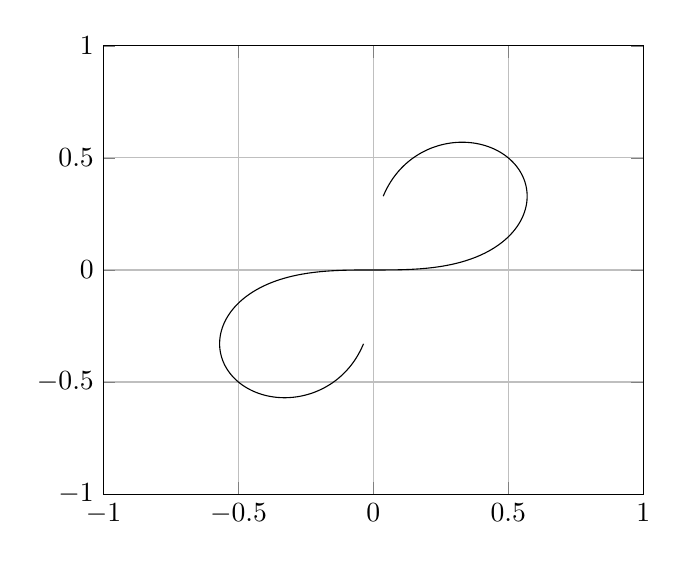
\begin{tikzpicture}
            \begin{axis}[
                xmin=-1,xmax=1,
                ymin=-1,ymax=1,
                grid=both,
                ]
                \addplot [domain=-3:3,samples=500]({x/(1+x^4)},{x^3/(1+x^4)}); 
            \end{axis}
        \end{tikzpicture}
        \caption{Representación Lemniscata.}
        \label{fig:lemniscata}
    \end{figure}

    Engañosamente: 
    \[
        \forall t \in \mathbb{R},\ \exists \left( t - \varepsilon, t + \varepsilon \right) = I_{\varepsilon}: f| : I_{\varepsilon} \rightarrow f\left( I_{\varepsilon} \right) 
    \]
    es homeomorfismo.

    En $t = 0, f\left( I_{\varepsilon} \right)$ \underline{no} es entorno de $f\left( 0 \right) = \left( 0, 0 \right)$, porque se tienen que tomar elementos de la rama ``vertical''.

    \item Las coordenadas polares $\left( 0, \rightarrow \right) \times \mathbb{R}^{} \rightarrow \mathbb{R}^{2},\ \left( r, \theta \right) \mapsto \left( r\cos \theta, r \sin \theta \right)$ es homeomorfismo local con $\theta_0 \in \left( \theta_0 - \pi, \theta_0 + \pi \right)$ hasta $\mathbb{R}^{2} \setminus L$ con $L$ la recta entre $O$ y $\theta_0$.
\end{enumerate} 
\end{ej}

\begin{defi}
Una \underline{variedad topológica} de $\dim m$ es un espacio localmente homeomorfo a $\mathbb{R}^m$, es decir, cada punto tiene un entorno abierto homeomorfo a una bola $B\left( 0, \varepsilon \right) \subset \mathbb{R}^m$ (luego a cualquier bola, luego a todo $\mathbb{R}^m$).
\end{defi}
\begin{ej}
Esferas, espacios proyectivos, toros...
\end{ej}

